\documentclass[dvipdfmx,cjk,xcolor=dvipsnames,envcountsect,notheorems,12pt]{beamer}
% * 16:9 のスライドを作るときは,aspectratio=169 を documentclass のオプションに追加する
% * 印刷用の配布資料を作るときは handout を documentclass のオプションに追加する
% (overlay が全て一つのスライドに出力される)

%\usepackage{pxjahyper}% しおりの文字化け対策 (なくても良い)
\usepackage{amsmath,amssymb,amsfonts,amsthm,ascmac,cases,bm,pifont}
\usepackage{graphicx}
\usepackage{url}

\usepackage{proof}
% \usepackage{tikz}
% \usetikzlibrary{positioning}

\newcommand\fun[2]{\lambda{#1}.{#2}}
\newcommand\lam{\lambda}

\newcommand\Resetz{\textbf{reset0}}
\newcommand\Shiftz{\textbf{shift0}}
\newcommand\Throw{\textbf{throw}}
\newcommand\resetz[1]{\Resetz~{#1}}
\newcommand\shiftz[2]{\Shiftz~{#1}.{#2}}
\newcommand\throw[2]{\Throw~{#1}~{#2}}

\newcommand\cfun[2]{\underline{\lambda}{#1}.{#2}}
\newcommand\clam{\underline{\lambda}}

\newcommand\cResetz{\underline{\textbf{reset0}}}
\newcommand\cShiftz{\underline{\textbf{shift0}}}
\newcommand\cThrow{\underline{\textbf{throw}}}
\newcommand\cresetz[1]{\cResetz~{#1}}
\newcommand\cshiftz[2]{\cShiftz~{#1}\to{#2}}
\newcommand\cthrow[2]{\cThrow~{#1}~{#2}}

\newcommand\cLet{\underline{\textbf{let}}}
\newcommand\cIn{\underline{\textbf{in}}}
\newcommand\clet[3]{\cLet~{#1}={#2}~\cIn~{#3}}
\newcommand\csp[1]{\texttt{\%}{#1}}
\newcommand\code[1]{\texttt{<}{#1}\texttt{>}}

\newcommand\cbra{\texttt{<}}
\newcommand\cket{\texttt{>}}

\newcommand\codeT[2]{\langle{#1}\rangle^{#2}}
\newcommand\codeTs[2]{\langle{#1}\rangle{\textbf{\textasciicircum}{#2}}}
\newcommand\contT[2]{({#1} \Rightarrow {#2})}

\newcommand\ord{\ge}

\newcommand\too{\leadsto^*}
\newcommand\downtoo{\rotatebox{-90}{$\leadsto^*$}}
\newcommand\pink[1]{\textcolor{pink}{#1}}
\newcommand\red[1]{\textcolor{red}{#1}}
\newcommand\green[1]{\textcolor{DarkGreen}{#1}}
\newcommand\magenta[1]{\textcolor{magenta}{#1}}
\newcommand\blue[1]{\textcolor{blue}{#1}}

\newcommand\forin[2]{\textbf{for}~{#1}~\textbf{to}~{#2}~\textbf{in}}
\newcommand\fordo[2]{\textbf{for}~{#1}~\textbf{to}~{#2}~\textbf{do}}
\newcommand\cforin[2]{\underline{\textbf{for}}~{#1}~\underline{\textbf{to}}~{#2}~\underline{\textbf{in}}}
\newcommand\cfordo[2]{\underline{\textbf{for}}~{#1}~\underline{\textbf{to}}~{#2}~\underline{\textbf{do}}}
\newcommand\Let{\textbf{let}}
\newcommand\In{\textbf{in}}
\newcommand\cArray[1]{\underline{[{#1}]}}
\newcommand\cArrays[2]{\underline{[{#1}][{#2}]}}
\newcommand\aryset[3]{{#1}[{#2}]\leftarrow {#3}}
%\newcommand\caryset[3]{\underline{\textbf{aryset}}~{#1}~{#2}~{#3}}
\newcommand\caryset[3]{\underline{\textbf{set}}~{#1}~{#2}~{#3}}
\newcommand\set{\underline{\textbf{set}}}

\newcommand\ift[3]{\textbf{if}~{#1}~\textbf{then}~{#2}~\textbf{else}~{#3}}
\newcommand\iif{\textbf{if}}
\newcommand\then{\textbf{then}}
\newcommand\eelse{\textbf{else}}
\newcommand\cif[3]{\underline{\textbf{if}}~\code{{#1}}~\code{{#2}}~\code{{#3}}}
\newcommand\cIf{\underline{\textbf{if}}}

\newcommand\cPlus{\underline{\textbf{+}}}
\newcommand\cTimes{\underline{\textbf{$\times$}}}
\newcommand\cint{\underline{\textbf{int}}}
\newcommand\fix{\textbf{fix}}
\newcommand\cfix{\underline{\textbf{fix}}}

\newcommand\lto{\leadsto}
\newcommand\cat{\underline{@}}

\newcommand\ksubst[2]{\{{#1}\Leftarrow{#2}\}}

% スライドのテーマ
\usetheme{sumiilab}
% ベースになる色を指定できる
% \usecolortheme[named=Magenta]{structure}
% 数式の文字が細くて見難い時は serif の代わりに bold にしましょう
% \mathversion{bold}

%% ===============================================
%% スライドの表紙および PDF に表示される情報
%% ===============================================

%% 発表会の名前とか(省略可)
% \session{研究室ゼミ}
%% スライドのタイトル
\title{多段階let挿入を行うコード生成言語の\\
  型システムの設計}
%% 必要ならば,サブタイトルも
% \subtitle{}
%% 発表者のお名前
\author{\underline{{\large 大石純平}} \quad 亀山幸義}
%% 発表者の所属([] 内は短い名前)
% \institute[東北大学 住井・松田研]{東北大学 工学部 電気情報物理工学科\\住井・松田研究室}% 学部生
\institute[筑波大学 コンピュータサイエンス専攻]{筑波大学 コンピュータ・サイエンス専攻}% 院生
%% 発表する日
\date{2016/9/9 \\{\tiny 日本ソフトウェア科学会第33回大会}}

%% ===============================================
%% 自動挿入される目次ページの設定(削除しても可)
%% ===============================================

% section の先頭に自動挿入される目次ページ(削除すると,表示されなくなる)
\AtBeginSection[]{
  \begin{frame}
    \frametitle{アウトライン}
    \tableofcontents[sectionstyle=show/shaded,subsectionstyle=show/hide/hide]
  \end{frame}}
% subsection の先頭に自動挿入される目次ページ(削除すると,表示されなくなる)
% \AtBeginSubsection[]{
% \begin{frame}
%   \frametitle{アウトライン}
%   \tableofcontents[sectionstyle=show/shaded,subsectionstyle=show/shaded/hide]
% \end{frame}}

%% 現在の section 以外を非表示にする場合は以下のようにする

%% \AtBeginSection[]{
%% \begin{frame}
%%   \frametitle{アウトライン}
%%   \tableofcontents[sectionstyle=show/hide,subsectionstyle=show/show/hide]
%% \end{frame}}
%% \AtBeginSubsection[]{
%% \begin{frame}
%%   \frametitle{アウトライン}
%%   \tableofcontents[sectionstyle=show/hide,subsectionstyle=show/shaded/hide]
%% \end{frame}}

%% ===============================================
%% 定理環境の設定
%% ===============================================

\setbeamertemplate{theorems}[numbered]% 定理環境に番号を付ける
\theoremstyle{definition}
\newtheorem{definition}{定義}
\newtheorem{axiom}{公理}
\newtheorem{theorem}{定理}
\newtheorem{lemma}{補題}
\newtheorem{corollary}{系}
\newtheorem{proposition}{命題}

%% ===============================================
%% ソースコードの設定
%% ===============================================

\usepackage{listings,jlisting}
% \usepackage[scale=0.9]{DejaVuSansMono}

\definecolor{DarkGreen}{rgb}{0,0.5,0}
% プログラミング言語と表示するフォント等の設定
\lstset{
  language={[Objective]Caml},% プログラミング言語
  basicstyle={\ttfamily\small},% ソースコードのテキストのスタイル
  keywordstyle={\bfseries},% 予約語等のキーワードのスタイル
  commentstyle={},% コメントのスタイル
  stringstyle={},% 文字列のスタイル
  frame=trlb,% ソースコードの枠線の設定 (none だと非表示)
  numbers=none,% 行番号の表示 (left だと左に表示)
  numberstyle={},% 行番号のスタイル
  xleftmargin=5pt,% 左余白
  xrightmargin=5pt,% 右余白
  keepspaces=true,% 空白を表示する
  mathescape,% $ で囲った部分を数式として表示する ($ がソースコード中で使えなくなるので注意)
  % 手動強調表示の設定
  moredelim=[is][\itshape]{@/}{/@},
  moredelim=[is][\color{red}]{@r\{}{\}@},
  moredelim=[is][\color{blue}]{@b\{}{\}@},
  moredelim=[is][\color{DarkGreen}]{@g\{}{\}@},
  moredelim=[is][\color{Magenta}]{@m\{}{\}@},
}

%% ===============================================
%% 本文
%% ===============================================
\begin{document}
\frame[plain]{\titlepage}% タイトルページ

\section*{アウトライン}

% 目次を表示させる(section を表示し,subsection は隠す)
\begin{frame}
  \frametitle{アウトライン}
  \tableofcontents[sectionstyle=show,subsectionstyle=hide]
\end{frame}

\section{概要}

\begin{frame}
  \frametitle{概要}
  % 図にする?
  プログラムを生成するプログラミング言語(=\alert{コード生成言語})の安全性を保証する研究
  \begin{itemize}
  \item<2-> 効率的なコードの生成
  \item<3-> 安全性の保証
  \item<4-> [⇒] \alert{多段階let 挿入}を安全に扱うための型システムを構築
  \end{itemize}
\end{frame}

\section{研究の背景}
\subsection{段階的計算(コード生成)}
\begin{frame}
  \frametitle{段階的計算 (Staged Computation)}
  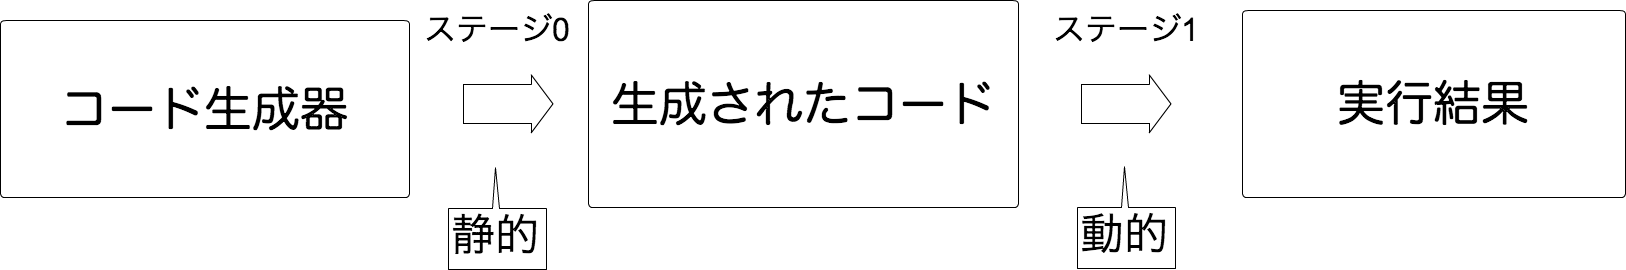
\includegraphics[clip,width=12cm]{./img/prggen.png}
  % この図を少し変更する
  \begin{itemize}
  \item コード生成ステージとコード実行ステージ
  \item[⇒] 段階的計算をサポートするプログラム言語 ⇒ コード生成言語
    % \item 生成するプログラムだけでなく,生成されたプログラムも型の整合性が静的に (生成前に) 保証される.
  \end{itemize}
\end{frame}

\subsection{コード生成の例}
\begin{frame}
  \frametitle{power関数のコード化}
  \begin{align*}
    \text{power} ~x~ ~n~ &~=~ x &\text{if} ~~n = 1 \\
                         &~~~\phantom{=}~ x * \text{power} ~x~ (n-1)~ &\text{if} ~~n > 1
  \end{align*}

  \pause
  $n = 8$に特化したコードの生成を行う
  \begin{align*}
    \text{gen\_power} ~x~ ~8~ =~ ~x~ * ~x~ * ~x~ * ~x~ * ~x~ * ~x~ * ~x~ * ~x~
  \end{align*}
  \pause
  $\text{gen\_power} ~x~ ~8~$ は$\text{power} ~x~ ~8~$ より高速
  \begin{itemize}
  \item 関数呼び出しがない
  \item 条件式がない
  \end{itemize}
\end{frame}

\subsection{段階的計算の課題}

\begin{frame}
  \frametitle{コード生成の利点と課題}
  % もっとコンパクトに

  利点
  \begin{itemize}
  \item \alert{「保守性・再利用性の高さ」}と\alert{「実行性能の高さ」}の両立
  \end{itemize}

  \pause

  課題
  \begin{itemize}
  \item パラメータに応じて,非常に多数のコードが生成される
    % \item 構文的,意味的に正しくないプログラムを生成しやすい
  \item 生成したコードのデバッグが容易ではない
  \item [⇒] \alert{コード生成の前に安全性を保証}したい
  \end{itemize}
\end{frame}

\begin{frame}
  \frametitle{従来研究}
  \begin{itemize}
  \item コード生成プログラムが,安全なコードのみを生成する事を静的に保証
    % \item<2-> let挿入等を実現する\alert{計算エフェクトを含む場合の安全性保証の研究は未整備}
  \item 安全なコード: 構文,型,変数束縛が正しいプログラム
  \end{itemize}

  \pause

  しかし\alert{多段階let挿入}等を実現する\alert{計算エフェクト}を含む場合のコード生成の安全性保証は研究途上
\end{frame}

\subsection{shift0/reset0}

\begin{frame}
  \frametitle{多段階let挿入}
  % 入れ子になったforループなどを飛び越えたコード移動を許す仕組みであり、ループ不変式の移動によって,効率的なコード生成に必要なプログラム技法

  \begin{itemize}
  \item 入れ子になったforループなどを飛び越えた\alert{コード移動}を許す仕組み
  \item ループ不変式の移動によって,\alert{効率的なコード生成}に必要なプログラミング技法
  \end{itemize}
\end{frame}

\begin{frame}[fragile]
  \frametitle{多段階let 挿入,let挿入の例}
  \begin{align*}
    & \forin{i = 0}{n} \\
    & ~~\forin{j = 0}{m} \\
    & ~~~~\magenta{\Let ~y ~= ~t ~\In} \\
    & ~~~~~~a[i][j] = b[i] + y \\
  \end{align*}

  % $\Rightarrow (\text{shift0/reset0 を付与})$

  \begin{onlyenv}<2>
    \begin{center}
      多段階let挿入\\
      $\Downarrow$
    \end{center}
    \begin{align*}
      & \magenta{\Let ~y ~= ~t ~\In} ~~~~~~~~~~\tiny{\text{--- t がi にも j にも依存しない式}} \\
      & ~~\forin{i = 0}{n} \\
      & ~~~~\forin{j = 0}{m} \\
      & ~~~~~~a[i][j] = b[i] + y \\
    \end{align*}
  \end{onlyenv}

  \begin{onlyenv}<3>
    \begin{center}
      普通のlet挿入\\
      $\Downarrow$
    \end{center}
    \begin{align*}
      & \forin{i = 0}{n} \\
      & ~~\magenta{\Let ~y ~= ~t ~\In} ~~~~~~~~~~\tiny{\text{--- t がi にのみ依存し jには依存しない式 }} \\
      & ~~~~\forin{j = 0}{m} \\
      & ~~~~~~a[i][j] = b[i] + y \\
    \end{align*}
  \end{onlyenv}

  \begin{onlyenv}<4>
    \begin{center}
      多段階let 挿入でも let挿入でもない\\
      $\Downarrow$
    \end{center}
    \begin{align*}
      & \forin{i = 0}{n} \\
      & ~~\forin{j = 0}{m} \\
      & ~~~~\magenta{\Let ~y ~= ~t ~\In} ~~~~~~~~~~\tiny{\text{--- t がi,j に依存した式 }} \\
      & ~~~~~~a[i][j] = b[i] + y \\
    \end{align*}
  \end{onlyenv}

\end{frame}

\subsection{限定継続}

\begin{frame}
  \frametitle{コントロールオペレータ}
  \begin{block}{プログラミング言語におけるプログラムを制御するプリミティブ}
    \begin{itemize}
    \item exception (例外): C++, Java, ML
    \item call/cc (第一級継続): Scheme, SML/NJ
    \item shift/reset (限定継続): Racket, Scala, OCaml
      \begin{itemize}
      \item 1989年以降多数研究がある
      \item コード生成におけるlet挿入が実現可能
        % \item shift/reset + コード生成の型システムが幾つか提案されている
      \end{itemize}
    \item \alert{shift0/reset0}
      \begin{itemize}
      \item 2011年以降研究が活発化.
      \item コード生成における\alert{多段階let挿入}が可能
      \end{itemize}
    \end{itemize}
  \end{block}
\end{frame}

%%% Local Variables:
%%% mode: japanese-latex
%%% TeX-master: "slide"
%%% End:
 % 問題 8分
% どうやって解くかの説明

\section{研究の目的}
\begin{frame}
  \frametitle{研究の目的}

  \begin{block}{\textbf{表現力}と\textbf{安全性}を兼ね備えたコード生成言語の構築}
    \begin{itemize}
    \item 表現力: 多段階let挿入,メモ化等の技法を表現
    \item 安全性: 生成されるコードの一定の性質を静的に検査
    \end{itemize}
  \end{block}

  \medskip
  \pause
  % 文字は減らしたほうが良さそう よりってのは何に比べて?
  \begin{block}{本研究: 簡潔で強力なコントロールオペレータに基づくコード生成体系の構築}
    \begin{itemize}
    \item コントロールオペレータ shift0/reset0 を利用し,let挿入などのコード生成技法を表現
    \item 型システムを構築して型安全性を保証
    \end{itemize}
  \end{block}
\end{frame}

\section{研究の内容}

\begin{frame}
  \center
  \huge{表現力を上げ(コードレベルでの多段階let挿入),安全性も保証するためにどうすればよいのか}
\end{frame}

% \subsection{本研究の手法}
% \begin{frame}
%   %   須藤さんの
%   \frametitle{本研究の手法}
%   %   \begin{itemize}
%   %   \item shift0/reset0 の型システムを単純化; let挿入等に絞る
%   %   \item これをコード生成言語の型システムに融合
%   %   \item 型システムの安全性を保証: Kameyama+ 2009, Sudo+2014 の手法を利用
%   %   \end{itemize}
%   \begin{columns}
%     \begin{column}{1.\textwidth}%% [横幅] 0.2\textwidth = ページ幅の 20 %
%       \center
%       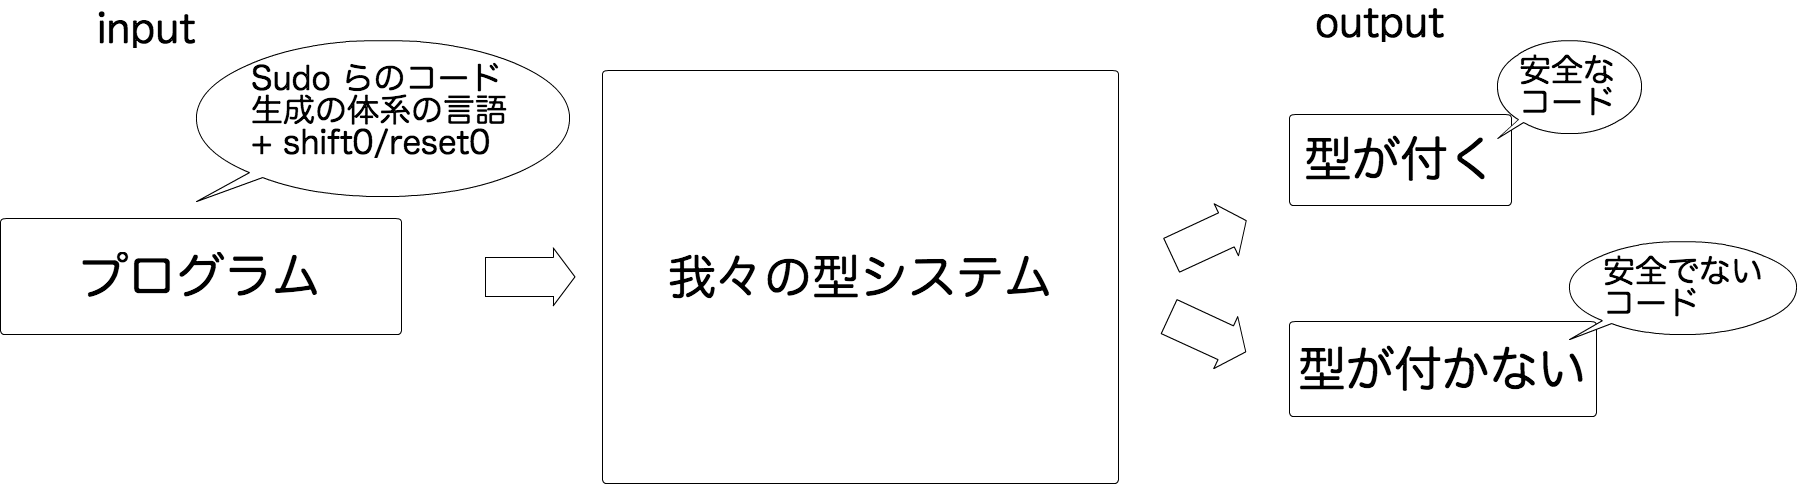
\includegraphics[clip,height=3.2cm]{./img/code_s0r0.png}
%     \end{column}
%   \end{columns}
% \end{frame}

\subsection{コード生成器と生成されるコード}

\begin{frame}
  \center
  \huge{まず表現力について}
\end{frame}

\begin{frame}
  \frametitle{let挿入の実現方法}

  \begin{visibleenv}<1->
    \begin{columns}
      \begin{column}{0.5\textwidth}%% [横幅] 0.2\textwidth = ページ幅の 20 %
        コード生成器
        \begin{align*}
          & \red{\circ}~ \cfordo{x = e1}{e2} \\
          & ~~\red{\circ}~ \cfordo{y = e3}{e4} \\
          & ~~~~~~\caryset{\code{a}}{(x,y)}~ \red{\circ}~ \text{cc}
        \end{align*}
      \end{column}
      $\too$
      \begin{column}{0.5\textwidth}%% [横幅] 0.2\textwidth = ページ幅の 20 %
        生成されるコード
        \begin{align*}
          & \cbra \magenta{\Let ~u' ~= ~\text{cc}' ~\In} \\
          & ~~\fordo{x' = e1'}{e2'} \\
          & ~~~~\fordo{y' = e3'}{e4'} \\
          & ~~~~~~\aryset{a}{x',y'}{u'} \cket
        \end{align*}
      \end{column}
    \end{columns}
  \end{visibleenv}

  \begin{visibleenv}<2>
    \begin{exampleblock}{shift0/reset0の導入}
      $\red{\circ}$ のところに \red{shift0/reset0} を用いることで,多段階let挿入を行う
    \end{exampleblock}
  \end{visibleenv}
\end{frame}

\subsection{多段階let 挿入}

\begin{frame}
  \frametitle{shift0/reset0 によるlet挿入}
  \noindent
  \begin{align*}
    \uncover<3->{\Resetz ~(E[\Shiftz~ k \to e]) ~\leadsto~ e \ksubst{k}{E}}
  \end{align*}

  \noindent

  % \begin{align*}
  %   \text{コード生成器:}~~
  %   & \uncover<4->{\blue{\Resetz}} ~~\cfordo{x = e1}{e2} \\
  %   & ~~\uncover<2-3>{\blue{\Resetz}} ~~\cfordo{y = e3}{e4} \\
  %   & ~~~~\uncover<2->{\blue{\Shiftz}~\blue{k}~\to}~
  %   \magenta{\cLet~u=t~\cIn} \\
  %   & ~~~~~~\uncover<2->{(\blue{\Throw~k}}~(\caryset{a}{(x,y)}{u})
  %   \uncover<2->{)} \\
  %   &   \uncover<3,5->{\blue{k}}
  %   \only<3>{\Leftarrow ~~\cfordo{y = e3}{e4}~[\ ]}
  %   \only<5->{\Leftarrow ~~\cfordo{x = e1}{e2} ~~\cfordo{y = e3}{e4} ~~[\ ]} \\
  %   \text{生成コード:}~~
  %   & \uncover<3,5->{\cbra~}
  %   \only<3>{\fordo{x' = e1'}{e2'}} \only<5->{\magenta{\Let ~u' ~= ~t' ~\In}} \\
  %   & ~~
  %   \only<3>{\magenta{\Let ~u' ~= ~t' ~\In}} \only<5->{\fordo{x' = e1'}{e2'}} \\
  %   & ~~~~\uncover<3,5->{\fordo{y' = e3'}{e4'}} \\
  %   & ~~~~~~\uncover<3,5->{\aryset{a}{x',y'}{u'} ~\cket}
  % \end{align*}

  \begin{align*}
    \scriptsize{\text{コード生成器:}}~~
    & \uncover<2-3>{\blue{\Resetz}} \only<1-2>{~\cfordo{x = e1}{e2}} \uncover<3>{\green{~\cfordo{x = e1}{e2}}}\\
    & ~~~~~~~~~~~ \only<1-2>{\cfordo{y = e3}{e4}} \uncover<3>{\green{\cfordo{y = e3}{e4}}}\\
    & ~~~~~~~~~~~~ \only<1-2>{\set~a~(x,y)~} \only<3>{\green{\set~a~(x,y)}~} \only<4->{~~~~~~~~~~~~~~~} \only<1>{cc} \uncover<2-3>{\blue{\Shiftz~ k \to}} \uncover<2->{\magenta{\cLet~u = cc~\cIn}~ \blue{\Throw~ k}~ u \\}
    % & ~~~~~~~~~~~~~~~~~~~~~~~~~~~~~~~~\uncover<2->{\magenta{\cLet~u = cc~\cIn}~ \blue{\Throw~ k}~ u} \\
    & \uncover<3->{\blue{k} \Leftarrow ~~\green{\cfordo{x = e1}{e2}} \\
    & ~~~~~~~~~~~\green{\cfordo{y = e3}{e4}} \\
    & ~~~~~~~~~~~~~\green{\caryset{a}{(x,y)}{}} [\ ]} \\
    \uncover<5->{\scriptsize{\text{生成コード:}}~~}
    & \uncover<5->{\cbra~}
      \uncover<5->{\magenta{\Let ~u' ~= ~cc' ~\In}} \\
    & ~~~~\uncover<5->{\fordo{x' = e1'}{e2'}} \\
    & ~~~~~~\uncover<5->{\fordo{y' = e3'}{e4'}} \\
    & ~~~~~~~~\uncover<5->{\aryset{a}{x',y'}{u'} ~\cket}
  \end{align*}

  % \begin{align*}
  %   \scriptsize{\text{コード生成器:}}~~
  %   & \uncover<2->{\blue{\Resetz}}~ \only<1-2>{\cfordo{x = e1}{e2}} \only<3>{\green{\cfordo{x = e1}{e2}}}\\
  %   & ~~~~~~~~~~~\only<1-2>{\cfordo{y = e3}{e4}} \only<3>{\green{\cfordo{y = e3}{e4}}}\\
  %   & ~~~~~~~~~~~~\only<1-2>{\set~a~(x,y)~} \only<3>{\green{\set~a~(x,y)~}} \only<1>{cc} \only<2>{\blue{\Shiftz~ k \to} \magenta{\cLet~u = cc~\cIn}~ \blue{\Throw~ k}~ u} \only<3->{\magenta{\cLet~u = cc~\cIn}~ \blue{\Throw~ k}~ u}\\
  %   %   & ~~~~~~~~~~~~~~~~~~~~~~~~~~~~~~~~\uncover<2->{\magenta{\cLet~u = cc~\cIn}~ \blue{\Throw~ k}~ u} \\
  %   & \uncover<3->{\blue{k} \Leftarrow ~~ \green{\cfordo{x = e1}{e2}} \\
  %   & ~~~~~~~~~~~\green{\cfordo{y = e3}{e4}} \\
  %   & ~~~~~~~~~~~~~\green{\caryset{a}{(x,y)}{}} [\ ]} \\
  %   \uncover<4->{\scriptsize{\text{生成コード:}}~~}
  %   & \uncover<4->{\cbra~}
  %   \uncover<4->{\magenta{\Let ~u' ~= ~cc' ~\In}} \\
  %   & ~~~~\uncover<4->{\fordo{x' = e1'}{e2'}} \\
  %   & ~~~~~~\uncover<4->{\fordo{y' = e3'}{e4'}} \\
  %   & ~~~~~~~~\uncover<4->{\aryset{a}{x',y'}{u'} ~\cket}
  % \end{align*}
\end{frame}


\begin{frame}
  \frametitle{shift0/reset0 による\alert{多段階}let挿入}
  \noindent
  \begin{align*}
    \Resetz ~(E[\Shiftz~ k \to e]) ~\leadsto~ e \ksubst{k}{E}
  \end{align*}

  \noindent
  % \begin{align*}
  %   \text{コード生成器:}~~
  %   & \red{\Resetz} ~~\cfordo{x = e1}{e2} \\
  %   & ~~\blue{\Resetz} ~~\cfordo{y = e3}{e4} \\
  %   & ~~~~\blue{\Shiftz}~\blue{k_2}~\to~
  %   \red{\Shiftz}~\red{k_1}~\to~
  %   \magenta{\cLet~u=t~\cIn} \\
  %   & ~~~~~~\red{\Throw~k_1}~
  %   (\blue{\Throw~k_2}~(\caryset{a}{(x,y)}{u})) \\
  %     %   & \red{k_1} \Leftarrow ~~\cfordo{x = e1}{e2}~[\ ] \\
  %     %   & \blue{k_2} \Leftarrow ~~\cfordo{y = e3}{e3}~[\ ] \\
  %   \text{生成コード:}~~
  %   & \cbra~\magenta{\Let ~u' ~= ~t' ~\In} \\
  %   & ~~\fordo{x' = e1'}{e2'} \\
  %   & ~~~~\fordo{y' = e3'}{e4'} \\
  %   & ~~~~~~\aryset{a}{x',y'}{u'} ~\cket
  % \end{align*}

  \begin{align*}
    \scriptsize{\text{コード生成器:}}~~
    & \red{\Resetz} ~~\cfordo{x = e1}{e2} \\
    & ~~\blue{\Resetz} ~~\cfordo{y = e3}{e4} \\
    & ~~~~ \caryset{a}{(x,y)}{\blue{\Shiftz~ k_1 \to}~ \magenta{\cLet~ u = cc1~ \cIn~} \blue{\Throw~ k_1}~ u;} \\
    & ~~~~ \set~ b~ (x,y)~ \blue{\Shiftz~ k_1 \to~} \red{\Shiftz~ k_2 \to}~ \\
    & ~~~~~~~~~~~~~~~~~~~~~~~~ \magenta{\cLet~ w = cc2~ \cIn~} \red{\Throw~ k_2} (\blue{\Throw~ k_1}~ w) \\
    % & \red{k_1} \Leftarrow ~~\cfordo{x = e1}{e2}~[\ ] \\
    % & \blue{k_2} \Leftarrow ~~\cfordo{y = e3}{e3}~[\ ] \\
    \uncover<2->{\scriptsize{\text{生成コード:}}~~}
    & \uncover<2->{\cbra~\magenta{\Let ~w' ~= ~cc2' ~\In}} \\
    & \uncover<2->{~~~~\fordo{x' = e1'}{e2'}} \\
    & \uncover<2->{~~~~~~\magenta{\Let ~u' ~= ~cc1' ~\In}} \\
    & \uncover<2->{~~~~~~~~\fordo{y' = e3'}{e4'}} \\
    & \uncover<2->{~~~~~~~~\aryset{a}{x',y'}{u'}} \\
    & \uncover<2->{~~~~~~~~\aryset{b}{x',y'}{w'} ~\cket}
  \end{align*}
\end{frame}

\begin{frame}
  \center
  \huge{次に安全性}
\end{frame}

\begin{frame}
  \center
  \huge{コード生成前の段階で,安全なコードかどうかを判断する}
\end{frame}

% \begin{frame}
%   \center
%   \huge{安全なコードにのみ型をつけるにはどうすればよいか}
% \end{frame}

\subsection{型システム}

\begin{frame}
  \frametitle{環境識別子(EC)を利用したスコープ表現\tiny{[Sudo+2014]}}
  % \begin{center}
  %   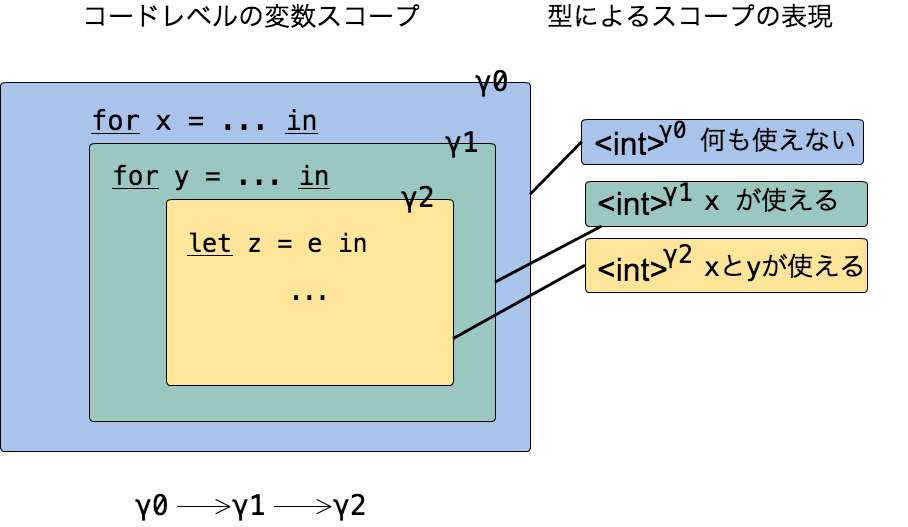
\includegraphics[clip,height=5.7cm]{./img/ec_for.png}
  % \end{center}
  % \begin{flushright}
  %   $\gamma_i ... \text{Refined Environment Classifier}$
  % \end{flushright}

  \newcommand\ml{\multicolumn}
  \center
  {\Large
    \begin{tabular}{l|l|l|l|l|l|}
      \cline{2-6}
      \alert{$\mathbf \gamma0$} & \ml{5}{|l|}{$\cfordo{x = e1}{e2}~~~~~~~~~~~~~~~$} \\ \cline{3-5}
                                & \alert{$\mathbf \gamma1$} & \ml{3}{|l|}{$\cfordo{y = e3}{e4}$} & \\ \cline{4-4}
                                &           & \alert{$\mathbf \gamma2$} & \ml{1}{|l|}{$\caryset{a}{(x,y)} cc$} & ~~ & \\ \cline{4-4}
                                &           & \ml{3}{|l|}{\ }    &               \\ \cline{3-5}
                                & \ml{5}{|l|}{~~~~~~~~~~~~~~~~~~ } \\ \cline{2-6}
    \end{tabular}
  }

  \begin{center}
    \begin{tabular}{c|c}
      スコープ & 使えるコード変数 \\ \hline
      \red{$\gamma0$} & なし \\ \hline
      \red{$\gamma1$} & $x$ \\ \hline
      \red{$\gamma2$} & $x, y$
    \end{tabular}\qquad
  \end{center}

  \red{$\gamma2$} $\ord$ \red{$\gamma1$} $\ord$ \red{$\gamma0$}
\end{frame}

\begin{frame}
  \frametitle{環境識別子(EC)を利用したスコープ表現\tiny{[Sudo+2014]}}
  % 大なり記号はスコープの大きさを表しているのではなく,使える自由変数の集合の大きさを表している
  型システムでコード変数のスコープを表現:

  \center
  \begin{align*}
    & \Gamma = \gamma2 \ord \gamma1,~
      x : \codeTs{\textbf{int}}{\gamma1},~
      y : \codeTs{\textbf{int}}{\gamma2}
  \end{align*}

  \begin{tabular}{c|c}
    $\gamma1$ & $\gamma2$ \\ \hline \hline
    \uncover<1->{$\Gamma ~\vdash~ x : \codeTs{\textbf{int}}{\gamma1}~~ \alert{\text{OK}}$} & \uncover<1->{$\Gamma ~\vdash~ x : \codeTs{\textbf{int}}{\gamma2}~~ \alert{\text{OK}}$} \\ \hline

    \uncover<1->{$\Gamma ~\vdash~ y : \codeTs{\textbf{int}}{\gamma1}~~ \alert{\text{NG}}$} & \uncover<1->{$\Gamma ~\vdash~ y : \codeTs{\textbf{int}}{\gamma2}~~ \alert{\text{OK}}$} \\ \hline

    \uncover<1->{$\Gamma ~\vdash~ x\cPlus y : \codeTs{\textbf{int}}{\gamma1}~~  \alert{\text{NG}}$} & \uncover<1->{$\Gamma ~\vdash~ x\cPlus y : \codeTs{\textbf{int}}{\gamma2}~~  \alert{\text{OK}}$}
  \end{tabular}

  \bigskip

  \begin{uncoverenv}<2->
    コードレベルのラムダ抽象の型付け規則で固有変数条件を利用:

    \[
      \infer[(\gamma_2~\text{is eigen var})]
      {\Gamma \vdash \cfun{x}{e} : \codeTs{t_1\to t_2}{\gamma_1} }
      {\Gamma,~\gamma_2 \ord \gamma_1,~x:\codeTs{t_1}{\gamma_2} \vdash
        e : \codeTs{t_2}{\gamma_2}}
    \]
  \end{uncoverenv}
\end{frame}

\begin{frame}
  \frametitle{環境識別子(EC)を利用したスコープ表現}

  先行研究:
  \begin{itemize}
  \item 局所的なスコープをもつ破壊的変数をもつコード生成の体系に対する(型安全な)型システムの構築
    [Sudo,Kiselyov,Kameyama 2014]
  \item グローバルなスコープをもつ破壊的変数への拡張
    [Kiselyov,Kameyama,Sudo 2016]
  \item[◯] コントロールオペレータには非対応
  \end{itemize}

  \medskip
  \begin{uncoverenv}<2->
    \begin{exampleblock}{問題点:}
      shift0/reset0 などのコントロールオペレータは,スコープの包含関係を逆転させてしまう.
    \end{exampleblock}
  \end{uncoverenv}
\end{frame}

\begin{frame}
  \center
  \huge{環境識別子(EC)の問題点}
\end{frame}


% \begin{frame}
%   \frametitle{環境識別子(EC)の問題点}
%   %   sudo らの研究の EC を素朴に適用させると問題があるということ言うスライド
%   %   ここに,forループとshift0/reset0 の例を再掲する.
%   %   もとのスライドの 24ページの絵をかく.

%   \newcommand\ml{\multicolumn}

%   \begin{uncoverenv}<1->
%     コード生成器:\\
%     \begin{tabular}{l|l|l|l|l|l|}
%       \cline{2-6}
%       & \ml{5}{|l|}{\cfordo{x = e1}{e2}~~~~~~~~~~~~~~~} \\ \cline{3-5}
%       & \footnotesize{\alert{$\mathbf \gamma0$}} & \ml{3}{|l|}{\Resetz~ \cfordo{y = e3}{e4}} & \\ \cline{4-4}
%       &           & \footnotesize{\alert{$\mathbf \gamma1$}} & \ml{1}{|l|}{\caryset{a}{(x,y)}{\Shiftz~ k $\to$ \footnotesize{\alert{$\mathbf \gamma2$}} {\large $\mid$} \magenta{\cLet~ u = cc \cIn}~ \footnotesize{\alert{$\mathbf \gamma3$}} {\large  $\mid$} \Throw~ k u}} & ~~ & \\ \cline{4-4}
%       &           & \ml{3}{|l|}{\ }    &               \\ \cline{3-5}
%       & \ml{5}{|l|}{~~~~~~~~~~~~~~~~~~ } \\ \cline{2-6}
%     \end{tabular}
%   \end{uncoverenv}

%   \begin{uncoverenv}<2>
%     生成コード:\\
%     \begin{tabular}{l|l|l|l|l|l|l|l|l|l|l|l|l|}
%       \cline{2-10}
%       & \ml{9}{|l|}{$\fordo{x' = e1'}{e2'}$~~~~~~~~~~~~~~~} \\ \cline{3-9}
%       & \footnotesize{\alert{$\mathbf \gamma0$}} & \ml{7}{|l|}{\magenta{$\Let~ u' = cc' ~ \In$}~} & \\ \cline{4-8}
%       & & \footnotesize{\alert{$\mathbf \gamma2$}} & \ml{5}{|l|}{$\fordo{y' = e3'}{e4'}$}  & & \\ \cline{5-7}
%       & & & \footnotesize{\alert{$\mathbf \gamma3$}} & \ml{3}{|l|}{\ }     &   &  &       \\ \cline{6-6}
%       & & & & \footnotesize{\alert{$\mathbf \gamma1$}} & \ml{1}{|l|}{$\aryset{a}{(x',y')}{u'}$} & & &  &  \\ \cline{6-6}
%       & & & & \ml{3}{|l|}{\ }  &   &   &           \\ \cline{5-7}
%       & & & \ml{5}{|l|}{\ } &  &               \\ \cline{4-8}
%       & & \ml{7}{|l|}{\ }  & \\ \cline{3-9}
%       & \ml{9}{|l|}{~~~~~~~ } \\ \cline{2-10}
%     \end{tabular}
%   \end{uncoverenv}

% \end{frame}

% \begin{frame}
%   \frametitle{環境識別子(EC)の問題点}
%   \center
%   コード生成器:
%   \begin{tabular}{c|c}
%     スコープ & 使えるコード変数 \\ \hline
%     \red{$\gamma0$} & x \\ \hline
%     \red{$\gamma1$} & x,y \\ \hline
%     \red{$\gamma2$} & x,y \\ \hline
%     \red{$\gamma3$} & x,y,u \\
%   \end{tabular}\qquad

%   \bigskip

%   生成コード:
%   \begin{tabular}{c|c}
%     スコープ & 使えるコード変数 \\ \hline
%     \red{$\gamma0$} & x \\ \hline
%     \red{$\gamma1$} & x,u \\ \hline
%     \red{$\gamma2$} & x,y,u \\ \hline
%     \red{$\gamma3$} & x,y,u \\
%   \end{tabular}\qquad

%   \begin{itemize}
%   \item 生成前と生成後の$\gamma1$ と $\gamma2$ の間には順序関係がない
%   \item $\gamma1$ $\cup$ $\gamma2$ = $\gamma3$
%   \end{itemize}
% \end{frame}

\begin{frame}
  \frametitle{コード生成前・後でスコープの包含関係が逆転}
  % sudo らの研究の EC を素朴に適用させると問題があるということ言うスライド
  % ここに,forループとshift0/reset0 の例を再掲する.
  % もとのスライドの 24ページの絵をかく.

  \newcommand\ml{\multicolumn}
  \begin{columns}
    \only<1>{コード生成器:}
    \begin{column}{0.6\textwidth}%% [横幅] 0.2\textwidth = ページ幅の 20 %
      \center
      \footnotesize
      \begin{tabular}{l|l|l|l|l|l|l|l|l|l|l}
        \cline{2-10}
        & \ml{9}{|l|}{$\cfordo{x = e1}{e2}$~~~~~~~~~~~~~~~} \\ \cline{3-9}
        & \footnotesize{\alert{$\mathbf \gamma0$}} & \ml{7}{|l|}{$\Resetz~ \cfordo{y = e3}{e4}$~} & \\ \cline{4-8}
        & & \footnotesize{\alert{$\mathbf \gamma1$}} & \ml{5}{|l|}{$\Shiftz~ k \to \magenta{\cLet~ u = cc ~ \cIn}$}  & & \\ \cline{5-7}
        & & & \footnotesize{\alert{$\mathbf \gamma2$}} & \ml{3}{|l|}{$\Throw~ k$}     &   &  &       \\ \cline{6-6}
        & & & & \footnotesize{\alert{$\mathbf \gamma3$}} & \ml{1}{|l|}{$\caryset{a}{(x,y)}{u}$} & & &  &  \\ \cline{6-6}
        & & & & \ml{3}{|l|}{\ }  &   &   &           \\ \cline{5-7}
        & & & \ml{5}{|l|}{\ } &  &               \\ \cline{4-8}
        & & \ml{7}{|l|}{\ }  & \\ \cline{3-9}
        & \ml{9}{|l|}{~~~~~~~ } \\ \cline{2-10}
      \end{tabular}
    \end{column}

    \begin{column}{0.5\textwidth}%% [横幅] 0.2\textwidth = ページ幅の 20 %
      \begin{onlyenv}<2->
        \flushright
        \footnotesize
        \begin{align*}
          \gamma3 \ord \red{\gamma2} \ord \red{\gamma1} \ord \gamma0 \\
        \end{align*}
      \end{onlyenv}

    \end{column}
  \end{columns}

  \bigskip

  \begin{columns}
    \only<1>{生成コード:~~}
    \begin{column}{0.6\textwidth}%% [横幅] 0.2\textwidth = ページ幅の 20 %
      \footnotesize
      \begin{tabular}{l|l|l|l|l|l|l|l|l|l|l|l|l|}
        \cline{2-10}
        & \ml{9}{|l|}{$\cbra$ $\fordo{x' = e1'}{e2'}$~~~~~~~~~~~~~~~} \\ \cline{3-9}
        & \footnotesize{\alert{$\mathbf \gamma0$}} & \ml{7}{|l|}{\magenta{$\Let~ u' = cc' ~ \In$}~} & \\ \cline{4-8}
        & & \footnotesize{\alert{$\mathbf \gamma2$}} & \ml{5}{|l|}{$\fordo{y' = e3'}{e4'}$}  & & \\ \cline{5-7}
        & & & \footnotesize{\alert{$\mathbf \gamma1$}} & \ml{3}{|l|}{\ }     &   &  &       \\ \cline{6-6}
        & & & & \footnotesize{\alert{$\mathbf \gamma3$}} & \ml{1}{|l|}{$\aryset{a}{(x',y')}{u'}$ $\cket$} & & &  &  \\ \cline{6-6}
        & & & & \ml{3}{|l|}{\ }  &   &   &           \\ \cline{5-7}
        & & & \ml{5}{|l|}{\ } &  &               \\ \cline{4-8}
        & & \ml{7}{|l|}{\ }  & \\ \cline{3-9}
        & \ml{9}{|l|}{~~~~~~~ } \\ \cline{2-10}
      \end{tabular}
    \end{column}

    \begin{column}{0.5\textwidth}%% [横幅] 0.2\textwidth = ページ幅の 20 %
      \begin{onlyenv}<2->
        \flushright
        \footnotesize
        \begin{align*}
          \gamma3 \ord \red{\gamma1} \ord \red{\gamma2} \ord \gamma0 \\
        \end{align*}
      \end{onlyenv}
    \end{column}
  \end{columns}
\end{frame}

% \begin{frame}
%   \frametitle{コード生成前・後でスコープの包含関係が逆転}
%   \smallskip
%   \center
%   コード生成器:
%   \begin{tabular}{c|c}
%     スコープ & 使えるコード変数? \\ \hline
%     \red{$\gamma0$} & $x$ \\ \hline
%     \red{$\gamma1$} & \uncover<1->{\blue{$x, y$}} \\ \hline %\uncover<2->{$\Rightarrow$ \red{$x, y, u$}} \\ \hline
%     \red{$\gamma2$} & \uncover<1->{\blue{$x, y, u$}} \\ \hline %\uncover<2->{$\Rightarrow$ \red{$x ,u$}}\\ \hline
%     \red{$\gamma3$} & $x, y, u$ \\
%   \end{tabular}\qquad

%   \bigskip

%   生成コード:
%   \begin{tabular}{c|c}
%     スコープ & 使えるコード変数? \\ \hline
%     \red{$\gamma0$} & $x'$ \\ \hline
%     \red{$\gamma2$} & \blue{$x', u'$} \\ \hline
%     \red{$\gamma1$} & \blue{$x', y', u'$} \\ \hline
%     \red{$\gamma3$} & $x', y', u'$ \\
%   \end{tabular}\qquad

%   \begin{itemize}
%   \item 生成前と生成後の$\gamma1$ と $\gamma2$ の間には順序関係がない
%     % \item $\gamma1$ $\cup$ $\gamma2$ = $\gamma3$
%   \item Sudo らの定義した環境識別子を素朴に使うと,型が合わない
%   \end{itemize}
% \end{frame}


% \begin{frame}
%   \frametitle{本研究での解決策}

%   3つのアイディア:
%   \begin{itemize}
%   \item 包含関係にないEC
%   \item ジョイン演算子
%   \item EC に関する多相性
%   \end{itemize}

% \end{frame}

\begin{frame}
  \center
  \huge{解決策}
\end{frame}

\begin{frame}
  \frametitle{本研究の解決策}
  \flushleft
  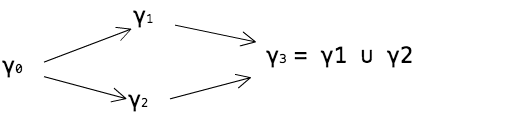
\includegraphics[clip,height=3cm]{./img/ecgraph.png}
  \begin{itemize}
  \item<2-> $\gamma1$ のコード変数は $\gamma2$ では使ってはいけない
  \item<2-> $\gamma2$ のコード変数は $\gamma1$ では使ってはいけない
  \item<3->[$\Rightarrow$] \red{$\gamma1$ と $\gamma2$ の間に順序を付けない}
  \end{itemize}

  \begin{itemize}
  \item<4-> $\gamma1, \gamma2$ のコード変数は $\gamma3$ で使ってよい
  \item<5->[$\Rightarrow$] \red{Sudoらの体系に $\cup$ (ユニオン) を追加} % ジョイン
  \end{itemize}
\end{frame}

\begin{frame}[fragile]
  \frametitle{コード生成+shift0/reset0 の型システム\small{ (の一部)}}
  reset0:
  \[
    \infer{\Gamma \vdash \resetz{e} : \codeTs{t}{\gamma} ~;~ \sigma}
    {\Gamma \vdash e : \codeTs{t}{\gamma} ~;~ \codeTs{t}{\gamma}, \sigma}
  \]

  shift0:
  \[
    \infer{\Gamma \vdash \shiftz{k}{e} : \codeTs{t1}{\red{\gamma1}} ~;~ \codeTs{t0}{\gamma0},\sigma}
    {\Gamma,~k:\contT{\codeTs{t1}{\gamma1}}{\codeTs{t0}{\gamma0}}
      \vdash e : \codeTs{t0}{\red{\gamma0}} ~;~ \sigma
      & \Gamma \models \gamma1 \ord \gamma0
    }
  \]

  throw:
  \[
    \infer
    {\Gamma,~k:\contT{\codeTs{t1}{\gamma1}}{\codeTs{t0}{\gamma0}}
      \vdash \throw{k}{v} : \codeTs{t0}{\gamma2} ~;~ \sigma}
    {\Gamma
      \vdash v : \codeTs{t1}{\red{\gamma1 \cup \gamma2}} ~;~ \sigma
      & \Gamma \models \gamma2 \ord \gamma0
    }
  \]
\end{frame}


%%% Local Variables:
%%% mode: japanese-latex
%%% TeX-master: "slide"
%%% End:
 % どうやって解くか 11分
%% 先の解決方法で実際になにができるのかの説明

\subsection{型付けの例}

% \begin{frame}
%   \frametitle{型が付く例/付かない例}
%   コード生成器
%   \begin{align*}
%     e & = \red{\Resetz} ~~\cfordo{i = 0}{n} \\
%     & \phantom{=}~~~~\blue{\Resetz} ~~\cfordo{j = 0}{m} \\
%     & \phantom{=}~~~~~~ \blue{\Shiftz}~\blue{k_2}~\to~ \red{\Shiftz}~\red{k_1}~\to~ \magenta{\cLet~y=\green{t}~\cIn} \\
%     & \phantom{=}~~~~~~~~ \red{k_1}~(\blue{k_2}~(\caryset{\code{a}}{(i,j)}{b[i] + y}))
%   \end{align*}

%   \pause
%   生成されるコード
%   \begin{columns}
%     \begin{column}{0.5\textwidth}%% [横幅] 0.2\textwidth = ページ幅の 20 %
%       \center
%       
\includegraphics[clip,height=1cm]{./img/batsu.png}
%       \begin{align*}
%         e & \too \magenta{\Let ~y ~= ~\green{a[i][j]} ~\In} \\
%           & \phantom{\too}~~~~ \fordo{i = 0}{n} \\
%           & \phantom{\too}~~~~~~\fordo{j = 0}{m} \\
%           & \phantom{\too}~~~~~~~~\aryset{a}{i,j}{b[i] + y} \\
%       \end{align*}
%     \end{column}

%     \begin{column}{0.5\textwidth}%% [横幅] 0.2\textwidth = ページ幅の 20 %
%       \center
%       
\includegraphics[height=1cm]{./img/maru.png}
%       \begin{align*}
%         e & \too \magenta{\Let ~y ~= ~\green{7} ~\In} \\
%           & \phantom{\too}~~~~ \fordo{i = 0}{n} \\
%           & \phantom{\too}~~~~~~\fordo{j = 0}{m} \\
%           & \phantom{\too}~~~~~~~~\aryset{a}{i,j}{b[i] + y} \\
%       \end{align*}
%     \end{column}
%   \end{columns}
% \end{frame}

\newcommand\boxterm{\framebox{
    \only<2>{\green{$\cint{3}$}}
    \only<3>{\red{$x~\cPlus~(\cint{3})$}}
    \phantom{A}
  }}

\begin{frame}
  \frametitle{型付けの例(1)}
  \begin{align*}
    e & = \Resetz ~~(\cfordo{x = e1}{e2} \\
       & \phantom{=}~~~ \Shiftz~k~\to~
         {\cLet~u=\green{\boxterm}~\cIn}~\Throw~k~u)
  \end{align*}

  \[
    \infer{\vdash e : \codeTs{t}{\gamma0};~\epsilon}
    {\infer[(\gamma1^*)]{\vdash \cfor{x=...} :
        \codeTs{t}{\gamma0};~\codeTs{t}{\gamma0}}
      {\infer{\gamma1 \ord \gamma0,~x:\codeTs{t}{\gamma1}
          \vdash \Shiftz~k~\to~... :
          \codeTs{t}{\gamma1};~\codeTs{t}{\gamma0}}
        {\infer[(\gamma2^*)]{\Gamma a \vdash \cLet~u=...:\codeTs{t}{\gamma0};~\epsilon}
          {\infer{\Gamma b \vdash
              \Throw~k~u:\codeTs{t}{\gamma2};~\epsilon }
            {\infer{\Gamma b \vdash
                u:\codeTs{t}{\gamma1 \cup \gamma2};~ \sigma}
              {}
            }
            &\infer*{\Gamma a \vdash
              \green{\boxterm}:\codeTs{t}{\red{\gamma0}};~\epsilon}
            {}
          }
        }
      }
    }
  \]

  % $[(\gamma1^*)]$ は eigen variable (固有変数)

  {\footnotesize
    \begin{align*}
      \Gamma a &= \gamma1 \ord \gamma0,~x:\codeTs{t}{\red{\gamma1}},
                ~k: \contT{\codeTs{t}{\gamma_1}}{\codeTs{t}{\gamma_0}} \\
      \Gamma b &= \Gamma a1,~\gamma2 \ord \gamma0,~u:\codeTs{t}{\gamma2}
    \end{align*}
  }

\end{frame}

\begin{frame}
  \frametitle{型付けの例(2)}

\newcommand\gammaa{\gamma1 \ord \gamma0,~x:\codeTs{t}{\gamma1}}
\newcommand\gammab{\Gamma a,\gamma2 \ord \gamma1,~y:\codeTs{t}{\gamma2}}
\newcommand\gammac{\Gamma b,\blue{k_2}:\contT{\codeTs{t}{\gamma2}}{\codeTs{t}{\gamma1}}}
\newcommand\gammad{\Gamma c,\red{k_1}:\contT{\codeTs{t}{\gamma1}}{\codeTs{t}{\gamma0}}}
\newcommand\gammae{\Gamma d,\gamma3 \ord \gamma0,\magenta{u}:\codeTs{t}{\gamma3}}

\footnotesize
  \begin{align*}
    e'= & \red{\Resetz}~(\cfordo{x = e1}{e2}~\blue{\Resetz} ~(\cfordo{y = e3}{e4} \\
       & \blue{\Shiftz}~\blue{k_2}\to~ \red{\Shiftz}~\red{k_1}\to~\magenta{\cLet~u=\green{X}~\cIn} 
         ~\red{\Throw~k_1}~(\blue{\Throw~k_2}~e5)))
  \end{align*}

  \[
    \infer{\vdash e'=\red{\Resetz}\cdots : \codeTs{t}{\gamma0};~~~\epsilon}
    {\infer[(\gamma1^*)]
      {\vdash \cfor{x=...} : \codeTs{t}{\gamma0};~~~\codeTs{t}{\gamma0}}
      {\infer{\Gamma a=\gammaa\vdash \blue{\Resetz}\cdots : \codeTs{t}{\gamma1};~~~\codeTs{t}{\gamma0}}
             {\infer[(\gamma2^*)]
                 {\Gamma a\vdash \cfor{y=...}: \codeTs{t}{\gamma1};~~~\codeTs{t}{\gamma1},\codeTs{t}{\gamma0}}
                 {\infer{\Gamma b=\gammab\vdash \blue{\Shiftz~k_2}... :\codeTs{t}{\gamma2}
                               ;~~~\codeTs{t}{\gamma1},\codeTs{t}{\gamma0}}
                        {\infer{\Gamma c=\gammac\vdash \red{\Shiftz~k_1}... :\codeTs{t}{\gamma1}
                                      ;~~~\codeTs{t}{\gamma0}}
                               {\infer[(\gamma3)]
                                  {\Gamma d=\gammad\vdash \magenta{\cLet~u=...} : \codeTs{t}{\gamma0};~~\epsilon}
                                  {\infer
                                     {\Gamma e=\gammae\vdash \red{\Throw~k_1}~... : \codeTs{t}{\gamma3};~~\epsilon}
                                     {\infer{\Gamma e\vdash \blue{\Throw~k_2}~e5 : 
                                               \codeTs{t}{\gamma1\cup\gamma3};~~\epsilon}
                                            {\infer*{\Gamma e\vdash e5:
                                               \codeTs{t}{\gamma2\cup\gamma1\cup\gamma3};~~~\epsilon}
                                                    {}
                                            }
                                     }
                                  &\infer*{\Gamma d\vdash X:\codeTs{t}{\gamma0};\epsilon}{}
                                  }
                               }
                        }
                 }
             }
      }
    }
  \]

\end{frame}

\section{まとめと今後の課題}

\begin{frame}
  \frametitle{まとめと今後の課題}
  まとめ
  \begin{itemize}
    % \item コードの言語にshift0 reset0 を組み込んだ言語の設計を行った
  \item コード生成言語の型システムに shift0/reset0 を組み込んだ 型システムの設計を完成させた.
  \item 安全なコードの場合に型が付くこと,安全でないコードの場合には型が付かないように意図通りに型システムが設計できていることをみた
  \end{itemize}

  % \vspace{1in}
  \vspace{\baselineskip}

  今後の課題
  \begin{itemize}
    % \item answer type modification に対応した型システムを設計し,(subject reduction 等の)健全性の証明を行う
  \item 設計した型システムの健全性の証明(Subject recudtion等)
  \item 型推論アルゴリズムの開発
  \item 言語の拡張
    \begin{itemize}
    \item グローバルな参照 (OCamlのlet ref)
    \item 生成したコードの実行 (MetaOCamlの run)
    \end{itemize}
  \end{itemize}
\end{frame}

%%% Local Variables:
%%% mode: japanese-latex
%%% TeX-master: "slide"
%%% End:
 % 何ができるか 型付けの例とか 5分


%%% Local Variables:
%%% mode: latex
%%% TeX-master: "slide_oishi"
%%% End:
 % 予備

\end{document}

%%% Local Variables:
%%% mode: japanese-latex
%%% TeX-master: t
%%% End:
